\documentclass[a4,8pt]{article}
\usepackage[margin=3cm,includefoot]{geometry}
\usepackage{siunitx}
\usepackage{fancyhdr}
\usepackage{tikz}
	\usetikzlibrary{arrows,shapes,positioning,calc}
\usepackage[font=it]{caption}
\usepackage{amsmath}

\pagestyle{fancy}
\lfoot{\sc Charlie Haddon}

\begin{document}

\begin{titlepage}
	\title{G484: Newtonian World}
	\author{Charlie Haddon}
	\date{}
	\pagenumbering{}
	\maketitle
	\vspace{15cm}
\end{titlepage}

\clearpage
\pagenumbering{arabic}

\section{General Motion}

\subsection{Newton's Laws of Motion}

Newton's three laws of motion are as follows:
\begin{enumerate}
	\item An object will remain at rest or move with constant velocity unless an external force acts upon it.
	\item The resultant force on an object is equal to its mass multiplied by its acceleration; $F=ma$ for constant mass.
	\item When a body exerts a force on another body, the second body simultaneously exerts an equal and opposite force on the original body.
\end{enumerate}


and some definitions of physical quantities:
\begin{itemize}
	\item Linear momentum, $p$ (\si{\kilo\gram\metre\per\square\second}), is defined as the product of the mass and velocity of an object and is a vector quantity.
	\item Net force, $F$ (\si{\newton}), on a body is equal to the rate of change of its momentum, $F=\frac{dp}{dt}$ or if the force is approximately constant, $F \approx \frac{\Delta p}{\Delta t}$
	\item Impulse, $J$ (\si{\newton\second}), is the integral of force over time or for constant force; force multipied by time and is therefore equal to the change in momentum, $mv-mu$.
\end{itemize}


\subsection{Collisions}
The principle of conservation of momentum states that the momentum of a system remains constant if no external force acts upon it. This princible is invaluable for calculating the velocities and masses in an n-body collision. For example, in a collision involving 2 bodies, $A$ and $B$:
$$m_A u_A + m_B u_B = m_A v_A + m_B v_B$$

\begin{figure}[h]
\begin{center}
Before collision:\\
\vspace{0.25cm}
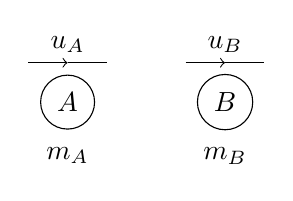
\begin{tikzpicture}[scale=1]
	\node[circle,draw] at (1,1) (A) {$A$};
	\node[below=0.1 of A] (1,1) {$m_A$}; 
	\draw[->] (0.5,1.5) -- (1,1.5) node[above] {$u_A$};  
	\draw (1,1.5) -- (1.5,1.5);

	\node[circle,draw] at (3,1) (B) {$B$};
	\node[below=0.1 of B] (3,1) {$m_B$}; 
	\draw[->] (2.5,1.5) -- (3,1.5) node[above] {$u_B$};  
	\draw (3,1.5) -- (3.5,1.5);
\end{tikzpicture}
\\
\vspace{0.5cm}

After collision:\\
\vspace{0.25cm}
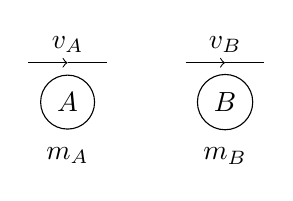
\begin{tikzpicture}[scale=1]
	\node[circle,draw] at (1,1) (A) {$A$};
	\node[below=0.1 of A] (1,1) {$m_A$}; 
	\draw[->] (0.5,1.5) -- (1,1.5) node[above] {$v_A$};  
	\draw (1,1.5) -- (1.5,1.5);

	\node[circle,draw] at (3,1) (B) {$B$};
	\node[below=0.1 of B] (3,1) {$m_B$}; 
	\draw[->] (2.5,1.5) -- (3,1.5) node[above] {$v_B$};  
	\draw (3,1.5) -- (3.5,1.5);
\end{tikzpicture}
\caption{Two objects collide and separate}
\end {center}
\end{figure}

or if the objects coalesce to form a single object, $C$:
$$m_A u_A + m_B u_B = (m_A + m_B) v_C$$

\begin{figure}[h]
\begin{center}
Before collision:\\
\vspace{0.25cm}
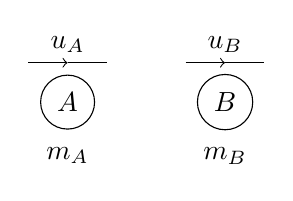
\begin{tikzpicture}[scale=1]
	\node[circle,draw] at (1,1) (A) {$A$};
	\node[below=0.1 of A] (1,1) {$m_A$}; 
	\draw[->] (0.5,1.5) -- (1,1.5) node[above] {$u_A$};  
	\draw (1,1.5) -- (1.5,1.5);

	\node[circle,draw] at (3,1) (B) {$B$};
	\node[below=0.1 of B] (3,1) {$m_B$}; 
	\draw[->] (2.5,1.5) -- (3,1.5) node[above] {$u_B$};  
	\draw (3,1.5) -- (3.5,1.5);
\end{tikzpicture}
\\
\vspace{0.5cm}

After collision:\\
\vspace{0.25cm}
\begin{tikzpicture}[scale=1]
	\node[circle,draw] at (1,1) (C) {$C$};
	\node[below=0.1 of A] (m) {$m_A + m_B$}; 
	\draw[->] (0.5,1.5) -- (1,1.5) node[above] {$v_C$};  
	\draw (1,1.5) -- (1.5,1.5);
\end{tikzpicture}
\caption{Two objects collide and coalesce}
\end{center}
\end{figure}

In a perfectly elastic collision, both momentum and kinetic energy are conserved, whereas in an inelastic collision, only momentum is conserved as some kinetic energy is lost to things like heat and sound etc.

\section{Circular Motion and Oscillations}
\subsection{Circular Motion}
A radian is the natural unit for measuring angles. A radian is defined as the angle subtended at the centre of a circle by an arc length equal to the circle's radius. One radian is equal to $\frac{180}{\pi}$ degrees.

\begin{figure}[h]
\begin{center}
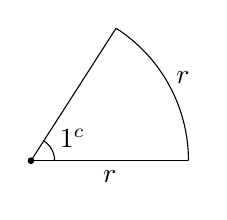
\begin{tikzpicture}
	\filldraw[black] (0,0) circle (1pt);
	\draw (0,0) -- (2,0);
	\draw (0,0) -- (1r:2);
	\draw (2,0) arc (0:1r:2);
	\draw (0.3,0) arc (0:1r:0.3);

	\node (theta) at (0.5r:0.6) {$1^c$};
	\node (r1) at (1,-0.2) {$r$};
	\node (r2) at (0.5r:2.2) {$r$};
\end{tikzpicture}
\caption{One radian}
\end{center}
\end{figure}

Circular motion is the result of a force acting perpendicular to an object's velocity, keeping the object at a fixed distance, $r$, from the origin. The general term for this force is centripetal force. An object undergoing circular motion is not in equilibrium as the resultant force is towards the centre of the circle, therefore the object is also accelerating towards the centre of the circle (centripetal acceleration). The speed of such an object is equal to $\frac{2\pi r}{T}$ where $r$ is the radius of the motion and $T$ is the time period (the time taken to complete a full cycle). The cetripetal acceleration is equal to $\frac{v^2}{r}$ where $v$ is the linear velocity calculated as before. Therefore, by Newton's second law, $F=ma$, centripetal force is equal to $\frac{mv^2}{r}$.

\begin{figure}[h]
\begin{center}
\begin{tikzpicture}
	\filldraw[black] (0,0) circle (1pt) node[below] {$O$};
	\draw[dashed] (60:2) arc (60:360:2);
	\draw (0:2) arc (0:60:2);
	\draw (0:2) -- (60:2);
	\node at ($(2,0) + (120:1) - (30:0.3)$) {$s$};
	\draw (0:0.3) arc (0:60:0.3);
	\node (theta) at (30:0.6) {$\delta\theta$};

	\draw (0,0) -- (2,0);
	\node at (1,-0.2) {$r$};
	\filldraw[black] (2,0) circle (1pt);
	\draw[->] (2,0) -- (2,1);
	\node at (2.3,0.5) {$v_0$};

	\draw (0,0) -- (60:2);
	\node at ($(60:1) + (150:0.2)$) {$r$};
	\filldraw[black] (60:2) circle (1pt);
	\draw[->] (60:2) -- ++(150:1);
	\node at ($(60:2) + (150:0.5) + (60:0.3)$) {$v_1$};
\end{tikzpicture}
\caption{Deriving the equation for centripetal acceleration}
\end{center}
\end{figure}

\subsection{Gravitational Fields}
A gravitational field is produced by all bodies with mass. By Newton's law of gravitation: Two bodies with mass exert a force on eachother proportional to the product of their masses and inversely proportional to the square of the distance between them. Gravitational field strength, $g$ (\si{\newton\per\kilo\gram}), is a measure of the force exerted on an object by a gravitational field per unit mass. Gravitational fields can be graphically represented using field lines showing the sources of gravitational field.

\begin{figure}[h]
\begin{center}
\begin{tikzpicture}
	\node[draw,circle] (O) at (0,0) {$m$};
	\foreach \theta in {0,45,90,135,180,225,270,315}
	{
		\draw (O) -- (\theta:1);
		\draw[->] (\theta:2) -- (\theta:1);
	}
\end{tikzpicture}
\caption{Gravitational field around a massive body}
\end{center}
\end{figure}

The constant of proportionality that relates gravitational force to mass and distance is $G$ and the equation for the force between two spherical or point masses is $F=-\frac{GMm}{r^2}$ where $M$ and $m$ are the masses of the two bodies and $r$ is the distance between them. By dividing throughout by one of the mass terms, the equation also gives the gravitational field strength of a point with distance $r$ from a mass: $g=-\frac{GM}{r^2}$. For large bodies like the Earth the gravitational field strength at the surface is approximately uniform. For the Earth this value is approximately equal to 9.81\si{\meter\per\square\second} (acceleration of free fall).

For an oscillating object or object in circular motion the time taken to complete a full cycle of motion is called a period. Kepler found by observation that that for all the planets in the solar system $T^2 \propto r^3$ where $T$ is the period of the planet's orbit and $r$ is its distance from Earth. This equation works only for objects in circular orbits and is dervied thusly:

By equating gravitational force and centripetal force:
$$\frac{GMm}{r^2} = \frac{mv^2}{r}$$

Dividing through by $m$ and multiplying by $r^2$:
$$GM = rv^2$$

Substituting in $v = \frac{2 \pi r}{T}$:
$$GM = r\left(\frac{2 \pi r}{T}\right)^2$$
$$\implies GM = \frac{4 {\pi}^2 r^3}{T^2}$$

And finally, rearranging for $T^2$:
$$T^2 = \left(\frac{4 {\pi}^2}{GM}\right)r^3$$

As $\frac{4 {\pi}^2}{GM}$ is constant:
$$T^2 \propto r^3$$

Satellites that orbit the Earth about the equator with a period of one day are called geostationary because they remain directly above the same point on the Earth at all times and are therefore stationary relative to Earth. This is particularly useful for communication satellites as it provides reliable coverage of a specific area meaning antannae don't need to track them and can be produced and maintained much more cheaply.

\end{document}
